Our dataset comprises of Quick,Draw! sketches and language descriptions of each semantically meaningful part in the sketch. The dataset contains 2 categories: face and angel, and these categories correspond directly to those in the original Quick!Draw! dataset. The part annotation comes from the SPG dataset \citep{spg_paper}. For the angel category, we annotate for the parts \textit{halo}, \textit{eyes}, \textit{nose}, \textit{mouth}, \textit{body}, \textit{outline of face}, and \textit{wings}. For the face category, we annotate for the parts \textit{eyes}, \textit{nose}, \textit{mouth}, \textit{hair}, \textit{outline of face}. 

\begin{figure*}[h]
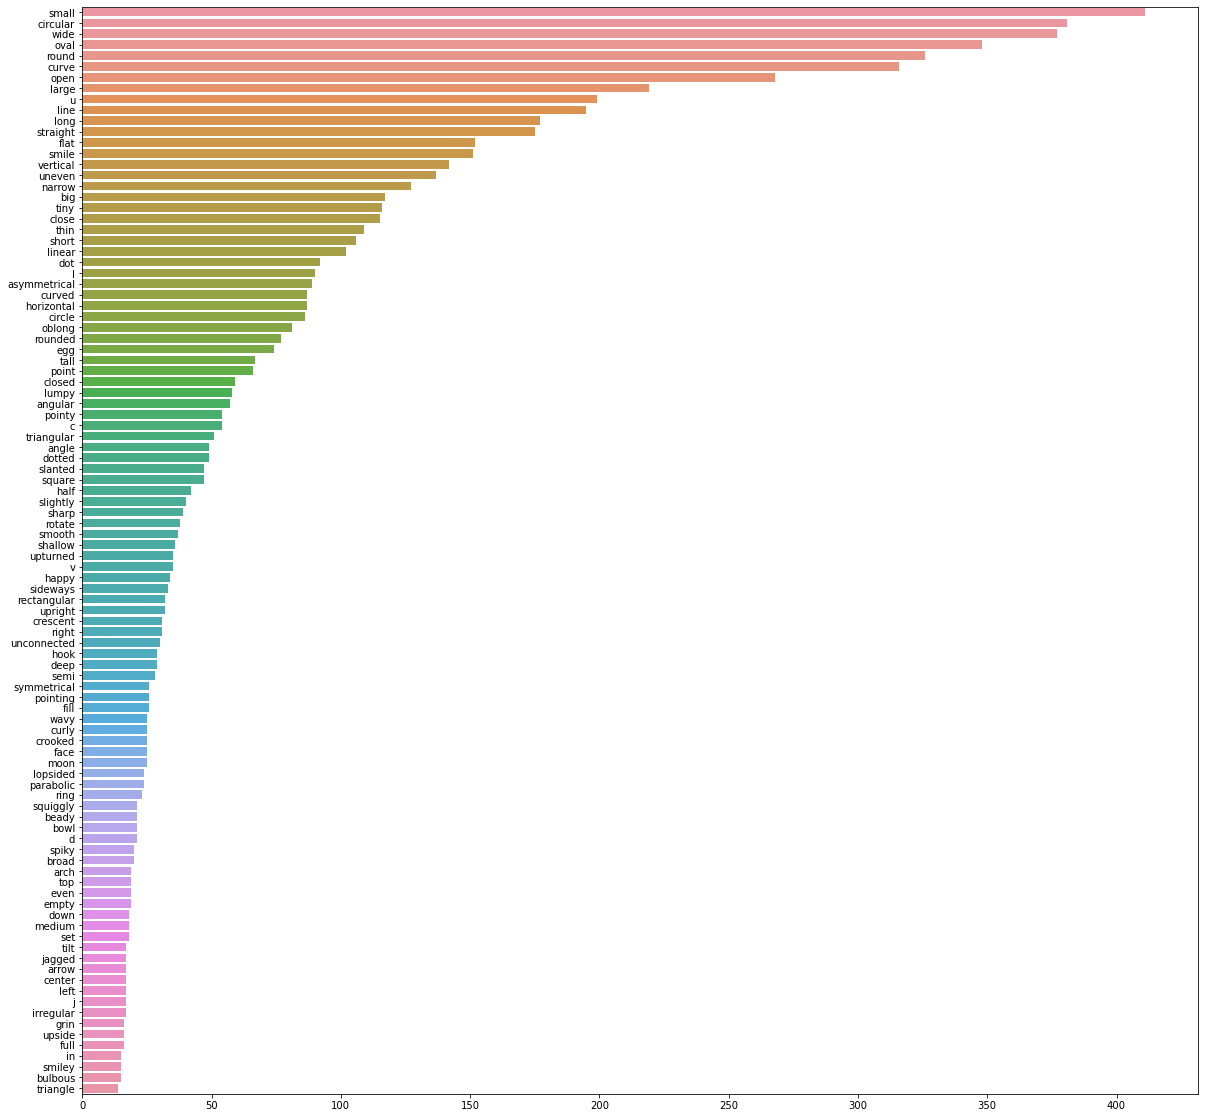
\includegraphics[width=\linewidth]{dataset_image/word_freq_face.png}  
\caption{Top 100 most frequent words in the dataset corpus.}
\label{word_freq}
\end{figure*}

\begin{table}[ht!]
\begin{minipage}{1\textwidth}
\begin{center}
{\small
\begin{tabular}{lrrr}
\toprule
~ & Face & Angel \\
\midrule
Number of constrastive pairs & 2515 & 3060 \\
Number of distinct words & 833 & 1107 \\
Number of sketches & 572 & 787 \\
\bottomrule
\end{tabular}}
\caption{Statistics of the dataset by category.}
\label{table:dataset_stats1}
\end{center}
\end{minipage}
\end{table}

\begin{table}[ht!]
\begin{minipage}{1\textwidth}
\begin{center}
{\small
\begin{tabular}{p{9em} | p{1.5em}p{1.5em}p{2em}p{1.5em}p{1.5em} | p{1.5em}p{1.5em}p{1.5em}p{2em}p{1.5em}p{1.5em}p{1.5em} }
\toprule
& \multicolumn{5}{c}{Face} & \multicolumn{7}{c}{Angel}\\
~ & eyes & nose & mouth & hair & face & halo & eyes & nose & mouth & face & body & wings  \\
\midrule
Number of sketches & 
334 & 572 & 572 & 104 & 572 &
558 & 114 & 8 & 80 & 732 & 781 & 779 \\
Number of distinct words & 
228 & 360 & 325 & 152 & 314 & 
365 & 112 & 21 & 88 & 379 & 425 & 534 \\
Number of constrastive pairs &
689 & 401 & 687 & 126 & 612 &
559 & 114 & 8 & 80 & 733 & 785 & 781 \\
\bottomrule
\end{tabular}}
\caption{Statistics of the dataset by sketch parts.}
\label{table:dataset_stats_byparts}
\end{center}
\end{minipage}
\end{table}

In Table \ref{table:dataset_stats_byparts}, we see some statistics about the dataset broken down by sketch parts, while in Table \ref{table:dataset_stats1}, we all list out the same statistics for the entire face and angel category. In general, we observe that compared to previous work that tend to have a fixed list of adjectives for each object parts, the descriptions in our dataset are free-form and non-constrainted. This characteristics is desirable and aligns with our goal to allow robot to collaborate smoothly with humans, since different people would describe the same things in very diverse ways. 